\documentclass[12pt]{article}
\usepackage[margin=1 in]{geometry}
\usepackage{graphicx}
\usepackage{float}
\usepackage{booktabs}
\usepackage{siunitx}
\usepackage{amsmath}
\usepackage{amssymb}


\title{Lab 10: LTSpice Analysis of Active Filters}
\author{Sean Balbale}
\date{November 11th, 2024}
\setlength{\parindent}{0in}

\begin{document}

\begin{titlepage}
	\begin{center}
		\vspace*{1in}

		\Huge
		\textbf{Lab 10}

		\LARGE
		LTSpice Analysis of Active Filters

		\vspace{3 in}

		\textbf{Student Name:} Sean Balbale
		\\ \textbf{Instructor:} Dr. Iman Salama
		\\ \textbf{Lab Partner Name:} Krish Gupta
		\\ \textbf{Date:} November 15, 2024

		\vfill


	\end{center}
\end{titlepage}

\newpage

\section{Introduction} 
Operational amplifiers (op-amps) have served as essential components in
electronic circuit design, particularly in sensing and signal processing
applications. This lab focused on constructing active filters with op-amps,
which are critical for biomedical applications such as electrocardiogram (EKG)
signal measurement. These filters were designed to amplify small signals while
selectively filtering out noise, thereby enhancing signal quality by rejecting
common-mode interference and removing unwanted frequency components. Through
LTSpice simulations, low-pass and high-pass filter designs were examined to
analyze their frequency responses, cutoff frequencies, and time-domain
performance. This approach provided insights into the role of active filters in
real-world signal processing, forming a foundation for practical applications in
biomedical and other electronic systems.



\section{Results}
% \begin{figure}[H]
% 	\centering
% 	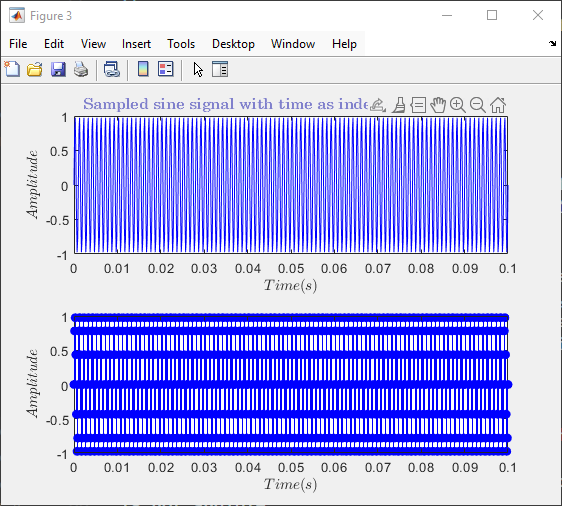
\includegraphics[width=0.3\textwidth]{fig 1f 7000.png}\hfill
% 	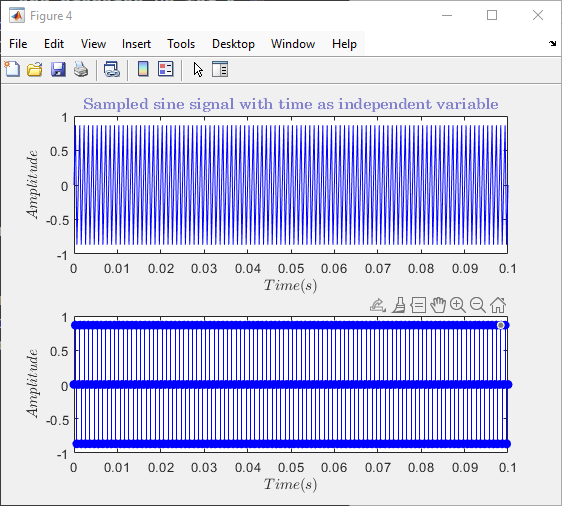
\includegraphics[width=0.3\textwidth]{fig 1f 3000.png}\hfill
% 	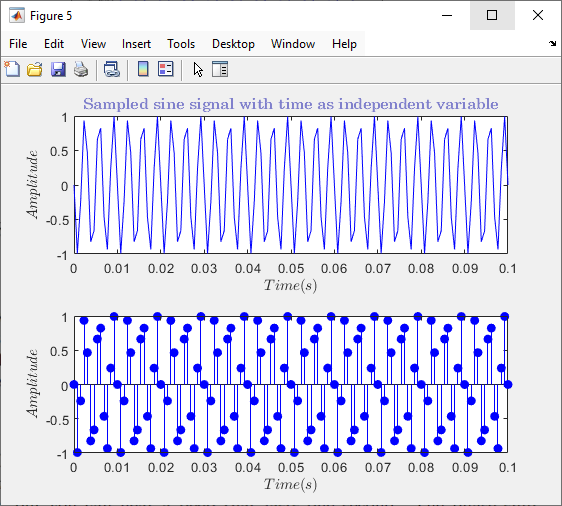
\includegraphics[width=0.3\textwidth]{fig 1f 1300.png}
% 	\caption{Sinusoidal with $f_s$ = 7 kHz, 3 kHz, and 1.3 kHz}
% 	\label{fig:fig3}
% % \end{figure}




\section{Discussion and Conclusion}


\section{References}
 [1] Dr. Iman Salama. “Lab 10 – LTSpice Analysis of Active Filters” Northeastern University. 11 November 2024.

\end{document}
